\documentclass[12pt]{article}

%packages
%\usepackage{latexsym}
\usepackage{graphicx}
\usepackage{color}
\usepackage{amsmath}
\usepackage{dsfont}
\usepackage{placeins}
\usepackage{amssymb}
\usepackage{wasysym}
\usepackage{abstract}
\usepackage{hyperref}
\usepackage{etoolbox}
\usepackage{datetime}
\usepackage{xcolor}
\usepackage{alphalph}
\usepackage{centernot}
\settimeformat{ampmtime}

%\usepackage{pstricks,pst-node,pst-tree}

%\usepackage{algpseudocode}
%\usepackage{amsthm}
%\usepackage{hyperref}
%\usepackage{mathrsfs}
%\usepackage{amsfonts}
%\usepackage{bbding}
%\usepackage{listings}
%\usepackage{appendix}
\usepackage[margin=1in]{geometry}
%\geometry{papersize={8.5in,11in},total={6.5in,9in}}
%\usepackage{cancel}
%\usepackage{algorithmic, algorithm}

\makeatletter
\def\maxwidth{ %
  \ifdim\Gin@nat@width>\linewidth
    \linewidth
  \else
    \Gin@nat@width
  \fi
}
\makeatother

\definecolor{fgcolor}{rgb}{0.345, 0.345, 0.345}
\newcommand{\hlnum}[1]{\textcolor[rgb]{0.686,0.059,0.569}{#1}}%
\newcommand{\hlstr}[1]{\textcolor[rgb]{0.192,0.494,0.8}{#1}}%
\newcommand{\hlcom}[1]{\textcolor[rgb]{0.678,0.584,0.686}{\textit{#1}}}%
\newcommand{\hlopt}[1]{\textcolor[rgb]{0,0,0}{#1}}%
\newcommand{\hlstd}[1]{\textcolor[rgb]{0.345,0.345,0.345}{#1}}%
\newcommand{\hlkwa}[1]{\textcolor[rgb]{0.161,0.373,0.58}{\textbf{#1}}}%
\newcommand{\hlkwb}[1]{\textcolor[rgb]{0.69,0.353,0.396}{#1}}%
\newcommand{\hlkwc}[1]{\textcolor[rgb]{0.333,0.667,0.333}{#1}}%
\newcommand{\hlkwd}[1]{\textcolor[rgb]{0.737,0.353,0.396}{\textbf{#1}}}%

\usepackage{framed}
\makeatletter
\newenvironment{kframe}{%
 \def\at@end@of@kframe{}%
 \ifinner\ifhmode%
  \def\at@end@of@kframe{\end{minipage}}%
  \begin{minipage}{\columnwidth}%
 \fi\fi%
 \def\FrameCommand##1{\hskip\@totalleftmargin \hskip-\fboxsep
 \colorbox{shadecolor}{##1}\hskip-\fboxsep
     % There is no \\@totalrightmargin, so:
     \hskip-\linewidth \hskip-\@totalleftmargin \hskip\columnwidth}%
 \MakeFramed {\advance\hsize-\width
   \@totalleftmargin\z@ \linewidth\hsize
   \@setminipage}}%
 {\par\unskip\endMakeFramed%
 \at@end@of@kframe}
\makeatother

\definecolor{shadecolor}{rgb}{.77, .77, .77}
\definecolor{messagecolor}{rgb}{0, 0, 0}
\definecolor{warningcolor}{rgb}{1, 0, 1}
\definecolor{errorcolor}{rgb}{1, 0, 0}
\newenvironment{knitrout}{}{} % an empty environment to be redefined in TeX

\usepackage{alltt}
\usepackage[T1]{fontenc}

\newcommand{\qu}[1]{``#1''}
\newcounter{probnum}
\setcounter{probnum}{1}

%create definition to allow local margin changes
\def\changemargin#1#2{\list{}{\rightmargin#2\leftmargin#1}\item[]}
\let\endchangemargin=\endlist 

%allow equations to span multiple pages
\allowdisplaybreaks

%define colors and color typesetting conveniences
\definecolor{gray}{rgb}{0.5,0.5,0.5}
\definecolor{black}{rgb}{0,0,0}
\definecolor{white}{rgb}{1,1,1}
\definecolor{blue}{rgb}{0.5,0.5,1}
\newcommand{\inblue}[1]{\color{blue}#1 \color{black}}
\definecolor{green}{rgb}{0.133,0.545,0.133}
\newcommand{\ingreen}[1]{\color{green}#1 \color{black}}
\definecolor{yellow}{rgb}{1,1,0}
\newcommand{\inyellow}[1]{\color{yellow}#1 \color{black}}
\definecolor{orange}{rgb}{0.9,0.649,0}
\newcommand{\inorange}[1]{\color{orange}#1 \color{black}}
\definecolor{red}{rgb}{1,0.133,0.133}
\newcommand{\inred}[1]{\color{red}#1 \color{black}}
\definecolor{purple}{rgb}{0.58,0,0.827}
\newcommand{\inpurple}[1]{\color{purple}#1 \color{black}}
\definecolor{backgcode}{rgb}{0.97,0.97,0.8}
\definecolor{Brown}{cmyk}{0,0.81,1,0.60}
\definecolor{OliveGreen}{cmyk}{0.64,0,0.95,0.40}
\definecolor{CadetBlue}{cmyk}{0.62,0.57,0.23,0}

%define new math operators
\DeclareMathOperator*{\argmax}{arg\,max~}
\DeclareMathOperator*{\argmin}{arg\,min~}
\DeclareMathOperator*{\argsup}{arg\,sup~}
\DeclareMathOperator*{\arginf}{arg\,inf~}
\DeclareMathOperator*{\convolution}{\text{\Huge{$\ast$}}}
\newcommand{\infconv}[2]{\convolution^\infty_{#1 = 1} #2}
%true functions

%%%% GENERAL SHORTCUTS

%shortcuts for pure typesetting conveniences
\newcommand{\bv}[1]{\boldsymbol{#1}}

%shortcuts for compound constants
\newcommand{\BetaDistrConst}{\dfrac{\Gamma(\alpha + \beta)}{\Gamma(\alpha)\Gamma(\beta)}}
\newcommand{\NormDistrConst}{\dfrac{1}{\sqrt{2\pi\sigma^2}}}

%shortcuts for conventional symbols
\newcommand{\tsq}{\tau^2}
\newcommand{\tsqh}{\hat{\tau}^2}
\newcommand{\sigsq}{\sigma^2}
\newcommand{\sigsqsq}{\parens{\sigma^2}^2}
\newcommand{\sigsqovern}{\dfrac{\sigsq}{n}}
\newcommand{\tausq}{\tau^2}
\newcommand{\tausqalpha}{\tau^2_\alpha}
\newcommand{\tausqbeta}{\tau^2_\beta}
\newcommand{\tausqsigma}{\tau^2_\sigma}
\newcommand{\betasq}{\beta^2}
\newcommand{\sigsqvec}{\bv{\sigma}^2}
\newcommand{\sigsqhat}{\hat{\sigma}^2}
\newcommand{\sigsqhatmlebayes}{\sigsqhat_{\text{Bayes, MLE}}}
\newcommand{\sigsqhatmle}[1]{\sigsqhat_{#1, \text{MLE}}}
\newcommand{\bSigma}{\bv{\Sigma}}
\newcommand{\bSigmainv}{\bSigma^{-1}}
\newcommand{\thetavec}{\bv{\theta}}
\newcommand{\thetahat}{\hat{\theta}}
\newcommand{\thetahatmle}{\hat{\theta}_{\mathrm{MLE}}}
\newcommand{\thetavechatmle}{\hat{\thetavec}_{\mathrm{MLE}}}
\newcommand{\muhat}{\hat{\mu}}
\newcommand{\musq}{\mu^2}
\newcommand{\muvec}{\bv{\mu}}
\newcommand{\muhatmle}{\muhat_{\text{MLE}}}
\newcommand{\lambdahat}{\hat{\lambda}}
\newcommand{\lambdahatmle}{\lambdahat_{\text{MLE}}}
\newcommand{\etavec}{\bv{\eta}}
\newcommand{\alphavec}{\bv{\alpha}}
\newcommand{\minimaxdec}{\delta^*_{\mathrm{mm}}}
\newcommand{\ybar}{\bar{y}}
\newcommand{\xbar}{\bar{x}}
\newcommand{\Xbar}{\bar{X}}
\newcommand{\phat}{\hat{p}}
\newcommand{\Phat}{\hat{P}}
\newcommand{\Zbar}{\bar{Z}}
\newcommand{\iid}{~{\buildrel iid \over \sim}~}
\newcommand{\inddist}{~{\buildrel ind \over \sim}~}
\newcommand{\approxdist}{~{\buildrel approx \over \sim}~}
\newcommand{\equalsindist}{~{\buildrel d \over =}~}
\newcommand{\loglik}[1]{\ell\parens{#1}}
\newcommand{\thetahatkminone}{\thetahat^{(k-1)}}
\newcommand{\thetahatkplusone}{\thetahat^{(k+1)}}
\newcommand{\thetahatk}{\thetahat^{(k)}}
\newcommand{\half}{\frac{1}{2}}
\newcommand{\third}{\frac{1}{3}}
\newcommand{\twothirds}{\frac{2}{3}}
\newcommand{\fourth}{\frac{1}{4}}
\newcommand{\fifth}{\frac{1}{5}}
\newcommand{\sixth}{\frac{1}{6}}

%shortcuts for vector and matrix notation
\newcommand{\A}{\bv{A}}
\newcommand{\At}{\A^T}
\newcommand{\Ainv}{\inverse{\A}}
\newcommand{\B}{\bv{B}}
\newcommand{\K}{\bv{K}}
\newcommand{\Kt}{\K^T}
\newcommand{\Kinv}{\inverse{K}}
\newcommand{\Kinvt}{(\Kinv)^T}
\newcommand{\M}{\bv{M}}
\newcommand{\Bt}{\B^T}
\newcommand{\Q}{\bv{Q}}
\renewcommand{\H}{\bv{H}}
\newcommand{\Qt}{\Q^T}
\newcommand{\R}{\bv{R}}
\newcommand{\Rt}{\R^T}
\newcommand{\Z}{\bv{Z}}
\newcommand{\X}{\bv{X}}
\newcommand{\U}{\bv{U}}
\newcommand{\V}{\bv{V}}
\newcommand{\Xsub}{\X_{\text{(sub)}}}
\newcommand{\Xsubadj}{\X_{\text{(sub,adj)}}}
\newcommand{\I}{\bv{I}}
\newcommand{\Y}{\bv{Y}}
\newcommand{\sigsqI}{\sigsq\I}
\renewcommand{\P}{\bv{P}}
\newcommand{\Psub}{\P_{\text{(sub)}}}
\newcommand{\Pt}{\P^T}
\newcommand{\Pii}{P_{ii}}
\newcommand{\Pij}{P_{ij}}
\newcommand{\IminP}{(\I-\P)}
\newcommand{\Xt}{\bv{X}^T}
\newcommand{\XtX}{\Xt\X}
\newcommand{\XtXinv}{\parens{\Xt\X}^{-1}}
\newcommand{\XtXinvXt}{\XtXinv\Xt}
\newcommand{\XXtXinvXt}{\X\XtXinvXt}
\newcommand{\x}{\bv{x}}
\newcommand{\w}{\bv{w}}
\renewcommand{\b}{\bv{b}}
\newcommand{\onevec}{\bv{1}}
\newcommand{\zerovec}{\bv{0}}
\newcommand{\oneton}{1, \ldots, n}
\newcommand{\yoneton}{y_1, \ldots, y_n}
\newcommand{\yonetonorder}{y_{(1)}, \ldots, y_{(n)}}
\newcommand{\Yoneton}{Y_1, \ldots, Y_n}
\newcommand{\iinoneton}{i \in \braces{\oneton}}
\newcommand{\onetom}{1, \ldots, m}
\newcommand{\jinonetom}{j \in \braces{\onetom}}
\newcommand{\xoneton}{x_1, \ldots, x_n}
\newcommand{\Xoneton}{X_1, \ldots, X_n}
\newcommand{\xt}{\x^T}
\newcommand{\y}{\bv{y}}
\newcommand{\yt}{\y^T}
\renewcommand{\c}{\bv{c}}
\newcommand{\ct}{\c^T}
\newcommand{\tstar}{\bv{t}^*}
\renewcommand{\u}{\bv{u}}
\renewcommand{\v}{\bv{v}}
\renewcommand{\a}{\bv{a}}
\newcommand{\s}{\bv{s}}
\newcommand{\yadj}{\y_{\text{(adj)}}}
\newcommand{\xjadj}{\x_{j\text{(adj)}}}
\newcommand{\xjadjM}{\x_{j \perp M}}
\newcommand{\yhat}{\hat{\y}}
\newcommand{\yhatsub}{\yhat_{\text{(sub)}}}
\newcommand{\yhatstar}{\yhat^*}
\newcommand{\yhatstarnew}{\yhatstar_{\text{new}}}
\newcommand{\z}{\bv{z}}
\newcommand{\zt}{\z^T}
\newcommand{\bb}{\bv{b}}
\newcommand{\bbt}{\bb^T}
\newcommand{\bbeta}{\bv{\beta}}
\newcommand{\beps}{\bv{\epsilon}}
\newcommand{\bepst}{\beps^T}
\newcommand{\e}{\bv{e}}
\newcommand{\Mofy}{\M(\y)}
\newcommand{\KofAlpha}{K(\alpha)}
\newcommand{\ellset}{\mathcal{L}}
\newcommand{\oneminalph}{1-\alpha}
\newcommand{\SSE}{\text{SSE}}
\newcommand{\SSEsub}{\text{SSE}_{\text{(sub)}}}
\newcommand{\MSE}{\text{MSE}}
\newcommand{\RMSE}{\text{RMSE}}
\newcommand{\SSR}{\text{SSR}}
\newcommand{\SST}{\text{SST}}
\newcommand{\JSest}{\delta_{\text{JS}}(\x)}
\newcommand{\Bayesest}{\delta_{\text{Bayes}}(\x)}
\newcommand{\EmpBayesest}{\delta_{\text{EmpBayes}}(\x)}
\newcommand{\BLUPest}{\delta_{\text{BLUP}}}
\newcommand{\MLEest}[1]{\hat{#1}_{\text{MLE}}}

%shortcuts for Linear Algebra stuff (i.e. vectors and matrices)
\newcommand{\twovec}[2]{\bracks{\begin{array}{c} #1 \\ #2 \end{array}}}
\newcommand{\threevec}[3]{\bracks{\begin{array}{c} #1 \\ #2 \\ #3 \end{array}}}
\newcommand{\fivevec}[5]{\bracks{\begin{array}{c} #1 \\ #2 \\ #3 \\ #4 \\ #5 \end{array}}}
\newcommand{\twobytwomat}[4]{\bracks{\begin{array}{cc} #1 & #2 \\ #3 & #4 \end{array}}}
\newcommand{\threebytwomat}[6]{\bracks{\begin{array}{cc} #1 & #2 \\ #3 & #4 \\ #5 & #6 \end{array}}}

%shortcuts for conventional compound symbols
\newcommand{\thetainthetas}{\theta \in \Theta}
\newcommand{\reals}{\mathbb{R}}
\newcommand{\complexes}{\mathbb{C}}
\newcommand{\rationals}{\mathbb{Q}}
\newcommand{\integers}{\mathbb{Z}}
\newcommand{\naturals}{\mathbb{N}}
\newcommand{\forallninN}{~~\forall n \in \naturals}
\newcommand{\forallxinN}[1]{~~\forall #1 \in \reals}
\newcommand{\matrixdims}[2]{\in \reals^{\,#1 \times #2}}
\newcommand{\inRn}[1]{\in \reals^{\,#1}}
\newcommand{\mathimplies}{\quad\Rightarrow\quad}
\newcommand{\mathlogicequiv}{\quad\Leftrightarrow\quad}
\newcommand{\eqncomment}[1]{\quad \text{(#1)}}
\newcommand{\limitn}{\lim_{n \rightarrow \infty}}
\newcommand{\limitN}{\lim_{N \rightarrow \infty}}
\newcommand{\limitd}{\lim_{d \rightarrow \infty}}
\newcommand{\limitt}{\lim_{t \rightarrow \infty}}
\newcommand{\limitsupn}{\limsup_{n \rightarrow \infty}~}
\newcommand{\limitinfn}{\liminf_{n \rightarrow \infty}~}
\newcommand{\limitk}{\lim_{k \rightarrow \infty}}
\newcommand{\limsupn}{\limsup_{n \rightarrow \infty}}
\newcommand{\limsupk}{\limsup_{k \rightarrow \infty}}
\newcommand{\floor}[1]{\left\lfloor #1 \right\rfloor}
\newcommand{\ceil}[1]{\left\lceil #1 \right\rceil}

%shortcuts for environments
\newcommand{\beqn}{\vspace{-0.25cm}\begin{eqnarray*}}
\newcommand{\eeqn}{\end{eqnarray*}}
\newcommand{\bneqn}{\vspace{-0.25cm}\begin{eqnarray}}
\newcommand{\eneqn}{\end{eqnarray}}

%shortcuts for mini environments
\newcommand{\parens}[1]{\left(#1\right)}
\newcommand{\squared}[1]{\parens{#1}^2}
\newcommand{\tothepow}[2]{\parens{#1}^{#2}}
\newcommand{\prob}[1]{\mathbb{P}\parens{#1}}
\newcommand{\cprob}[2]{\prob{#1~|~#2}}
\newcommand{\littleo}[1]{o\parens{#1}}
\newcommand{\bigo}[1]{O\parens{#1}}
\newcommand{\Lp}[1]{\mathbb{L}^{#1}}
\renewcommand{\arcsin}[1]{\text{arcsin}\parens{#1}}
\newcommand{\prodonen}[2]{\bracks{\prod_{#1=1}^n #2}}
\newcommand{\mysum}[4]{\sum_{#1=#2}^{#3} #4}
\newcommand{\sumonen}[2]{\sum_{#1=1}^n #2}
\newcommand{\infsum}[2]{\sum_{#1=1}^\infty #2}
\newcommand{\infprod}[2]{\prod_{#1=1}^\infty #2}
\newcommand{\infunion}[2]{\bigcup_{#1=1}^\infty #2}
\newcommand{\infinter}[2]{\bigcap_{#1=1}^\infty #2}
\newcommand{\infintegral}[2]{\int^\infty_{-\infty} #2 ~\text{d}#1}
\newcommand{\supthetas}[1]{\sup_{\thetainthetas}\braces{#1}}
\newcommand{\bracks}[1]{\left[#1\right]}
\newcommand{\braces}[1]{\left\{#1\right\}}
\newcommand{\set}[1]{\left\{#1\right\}}
\newcommand{\abss}[1]{\left|#1\right|}
\newcommand{\norm}[1]{\left|\left|#1\right|\right|}
\newcommand{\normsq}[1]{\norm{#1}^2}
\newcommand{\inverse}[1]{\parens{#1}^{-1}}
\newcommand{\rowof}[2]{\parens{#1}_{#2\cdot}}

%shortcuts for functionals
\newcommand{\realcomp}[1]{\text{Re}\bracks{#1}}
\newcommand{\imagcomp}[1]{\text{Im}\bracks{#1}}
\newcommand{\range}[1]{\text{range}\bracks{#1}}
\newcommand{\colsp}[1]{\text{colsp}\bracks{#1}}
\newcommand{\rowsp}[1]{\text{rowsp}\bracks{#1}}
\newcommand{\tr}[1]{\text{tr}\bracks{#1}}
\newcommand{\rank}[1]{\text{rank}\bracks{#1}}
\newcommand{\proj}[2]{\text{Proj}_{#1}\bracks{#2}}
\newcommand{\projcolspX}[1]{\text{Proj}_{\colsp{\X}}\bracks{#1}}
\newcommand{\median}[1]{\text{median}\bracks{#1}}
\newcommand{\mean}[1]{\text{mean}\bracks{#1}}
\newcommand{\dime}[1]{\text{dim}\bracks{#1}}
\renewcommand{\det}[1]{\text{det}\bracks{#1}}
\newcommand{\expe}[1]{\mathbb{E}\bracks{#1}}
\newcommand{\expeabs}[1]{\expe{\abss{#1}}}
\newcommand{\expesub}[2]{\mathbb{E}_{#1}\bracks{#2}}
\newcommand{\indic}[1]{\mathds{1}_{#1}}
\newcommand{\var}[1]{\mathbb{V}\text{ar}\bracks{#1}}
\newcommand{\cov}[2]{\mathbb{C}\text{ov}\bracks{#1, #2}}
\newcommand{\corr}[2]{\text{Corr}\bracks{#1, #2}}
\newcommand{\se}[1]{\mathbb{S}\text{E}\bracks{#1}}
\newcommand{\seest}[1]{\hat{\mathbb{S}\text{E}}\bracks{#1}}
\newcommand{\bias}[1]{\text{Bias}\bracks{#1}}
\newcommand{\derivop}[2]{\dfrac{\text{d}}{\text{d} #1}\bracks{#2}}
\newcommand{\partialop}[2]{\dfrac{\partial}{\partial #1}\bracks{#2}}
\newcommand{\secpartialop}[2]{\dfrac{\partial^2}{\partial #1^2}\bracks{#2}}
\newcommand{\mixpartialop}[3]{\dfrac{\partial^2}{\partial #1 \partial #2}\bracks{#3}}

%shortcuts for functions
\renewcommand{\exp}[1]{\mathrm{exp}\parens{#1}}
\renewcommand{\cos}[1]{\text{cos}\parens{#1}}
\renewcommand{\sin}[1]{\text{sin}\parens{#1}}
\newcommand{\sign}[1]{\text{sign}\parens{#1}}
\newcommand{\are}[1]{\mathrm{ARE}\parens{#1}}
\newcommand{\natlog}[1]{\ln\parens{#1}}
\newcommand{\oneover}[1]{\frac{1}{#1}}
\newcommand{\overtwo}[1]{\frac{#1}{2}}
\newcommand{\overn}[1]{\frac{#1}{n}}
\newcommand{\oneoversqrt}[1]{\oneover{\sqrt{#1}}}
\newcommand{\sqd}[1]{\parens{#1}^2}
\newcommand{\loss}[1]{\ell\parens{\theta, #1}}
\newcommand{\losstwo}[2]{\ell\parens{#1, #2}}
\newcommand{\cf}{\phi(t)}

%English language specific shortcuts
\newcommand{\ie}{\textit{i.e.} }
\newcommand{\AKA}{\textit{AKA} }
\renewcommand{\iff}{\textit{iff}}
\newcommand{\eg}{\textit{e.g.} }
\newcommand{\st}{\textit{s.t.} }
\newcommand{\wrt}{\textit{w.r.t.} }
\newcommand{\mathst}{~~\text{\st}~~}
\newcommand{\mathand}{~~\text{and}~~}
\newcommand{\ala}{\textit{a la} }
\newcommand{\ppp}{posterior predictive p-value}
\newcommand{\dd}{dataset-to-dataset}

%shortcuts for distribution titles
\newcommand{\logistic}[2]{\mathrm{Logistic}\parens{#1,\,#2}}
\newcommand{\bernoulli}[1]{\mathrm{Bernoulli}\parens{#1}}
\newcommand{\betanot}[2]{\mathrm{Beta}\parens{#1,\,#2}}
\newcommand{\stdbetanot}{\betanot{\alpha}{\beta}}
\newcommand{\multnormnot}[3]{\mathcal{N}_{#1}\parens{#2,\,#3}}
\newcommand{\normnot}[2]{\mathcal{N}\parens{#1,\,#2}}
\newcommand{\classicnormnot}{\normnot{\mu}{\sigsq}}
\newcommand{\stdnormnot}{\normnot{0}{1}}
\newcommand{\uniformdiscrete}[1]{\mathrm{Uniform}\parens{\braces{#1}}}
\newcommand{\uniform}[2]{\mathrm{U}\parens{#1,\,#2}}
\newcommand{\stduniform}{\uniform{0}{1}}
\newcommand{\geometric}[1]{\mathrm{Geometric}\parens{#1}}
\newcommand{\hypergeometric}[3]{\mathrm{Hypergeometric}\parens{#1,\,#2,\,#3}}
\newcommand{\exponential}[1]{\mathrm{Exp}\parens{#1}}
\newcommand{\gammadist}[2]{\mathrm{Gamma}\parens{#1, #2}}
\newcommand{\poisson}[1]{\mathrm{Poisson}\parens{#1}}
\newcommand{\binomial}[2]{\mathrm{Binomial}\parens{#1,\,#2}}
\newcommand{\negbin}[2]{\mathrm{NegBin}\parens{#1,\,#2}}
\newcommand{\rayleigh}[1]{\mathrm{Rayleigh}\parens{#1}}
\newcommand{\multinomial}[2]{\mathrm{Multinomial}\parens{#1,\,#2}}
\newcommand{\gammanot}[2]{\mathrm{Gamma}\parens{#1,\,#2}}
\newcommand{\cauchynot}[2]{\text{Cauchy}\parens{#1,\,#2}}
\newcommand{\invchisqnot}[1]{\text{Inv}\chisq{#1}}
\newcommand{\invscaledchisqnot}[2]{\text{ScaledInv}\ncchisq{#1}{#2}}
\newcommand{\invgammanot}[2]{\text{InvGamma}\parens{#1,\,#2}}
\newcommand{\chisq}[1]{\chi^2_{#1}}
\newcommand{\ncchisq}[2]{\chi^2_{#1}\parens{#2}}
\newcommand{\ncF}[3]{F_{#1,#2}\parens{#3}}

%shortcuts for PDF's of common distributions
\newcommand{\logisticpdf}[3]{\oneover{#3}\dfrac{\exp{-\dfrac{#1 - #2}{#3}}}{\parens{1+\exp{-\dfrac{#1 - #2}{#3}}}^2}}
\newcommand{\betapdf}[3]{\dfrac{\Gamma(#2 + #3)}{\Gamma(#2)\Gamma(#3)}#1^{#2-1} (1-#1)^{#3-1}}
\newcommand{\normpdf}[3]{\frac{1}{\sqrt{2\pi#3}}\exp{-\frac{1}{2#3}(#1 - #2)^2}}
\newcommand{\normpdfvarone}[2]{\dfrac{1}{\sqrt{2\pi}}e^{-\half(#1 - #2)^2}}
\newcommand{\chisqpdf}[2]{\dfrac{1}{2^{#2/2}\Gamma(#2/2)}\; {#1}^{#2/2-1} e^{-#1/2}}
\newcommand{\invchisqpdf}[2]{\dfrac{2^{-\overtwo{#1}}}{\Gamma(#2/2)}\,{#1}^{-\overtwo{#2}-1}  e^{-\oneover{2 #1}}}
\newcommand{\exponentialpdf}[2]{#2\exp{-#2#1}}
\newcommand{\poissonpdf}[2]{\dfrac{e^{-#1} #1^{#2}}{#2!}}
\newcommand{\binomialpdf}[3]{\binom{#2}{#1}#3^{#1}(1-#3)^{#2-#1}}
\newcommand{\rayleighpdf}[2]{\dfrac{#1}{#2^2}\exp{-\dfrac{#1^2}{2 #2^2}}}
\newcommand{\gammapdf}[3]{\dfrac{#3^#2}{\Gamma\parens{#2}}#1^{#2-1}\exp{-#3 #1}}
\newcommand{\cauchypdf}[3]{\oneover{\pi} \dfrac{#3}{\parens{#1-#2}^2 + #3^2}}
\newcommand{\Gammaf}[1]{\Gamma\parens{#1}}

%shortcuts for miscellaneous typesetting conveniences
\newcommand{\notesref}[1]{\marginpar{\color{gray}\tt #1\color{black}}}

%%%% DOMAIN-SPECIFIC SHORTCUTS

%Real analysis related shortcuts
\newcommand{\zeroonecl}{\bracks{0,1}}
\newcommand{\forallepsgrzero}{\forall \epsilon > 0~~}
\newcommand{\lessthaneps}{< \epsilon}
\newcommand{\fraccomp}[1]{\text{frac}\bracks{#1}}

%Bayesian related shortcuts
\newcommand{\yrep}{y^{\text{rep}}}
\newcommand{\yrepisq}{(\yrep_i)^2}
\newcommand{\yrepvec}{\bv{y}^{\text{rep}}}


%Probability shortcuts
\newcommand{\SigField}{\mathcal{F}}
\newcommand{\ProbMap}{\mathcal{P}}
\newcommand{\probtrinity}{\parens{\Omega, \SigField, \ProbMap}}
\newcommand{\convp}{~{\buildrel p \over \rightarrow}~}
\newcommand{\convLp}[1]{~{\buildrel \Lp{#1} \over \rightarrow}~}
\newcommand{\nconvp}{~{\buildrel p \over \nrightarrow}~}
\newcommand{\convae}{~{\buildrel a.e. \over \longrightarrow}~}
\newcommand{\convau}{~{\buildrel a.u. \over \longrightarrow}~}
\newcommand{\nconvau}{~{\buildrel a.u. \over \nrightarrow}~}
\newcommand{\nconvae}{~{\buildrel a.e. \over \nrightarrow}~}
\newcommand{\convd}{~{\buildrel \mathcal{D} \over \rightarrow}~}
\newcommand{\nconvd}{~{\buildrel \mathcal{D} \over \nrightarrow}~}
\newcommand{\withprob}{~~\text{w.p.}~~}
\newcommand{\io}{~~\text{i.o.}}

\newcommand{\Acl}{\bar{A}}
\newcommand{\ENcl}{\bar{E}_N}
\newcommand{\diam}[1]{\text{diam}\parens{#1}}

\newcommand{\taua}{\tau_a}

\newcommand{\myint}[4]{\int_{#2}^{#3} #4 \,\text{d}#1}
\newcommand{\laplacet}[1]{\mathscr{L}\bracks{#1}}
\newcommand{\laplaceinvt}[1]{\mathscr{L}^{-1}\bracks{#1}}
\renewcommand{\min}[1]{\text{min}\braces{#1}}
\renewcommand{\max}[1]{\text{max}\braces{#1}}

\newcommand{\Vbar}[1]{\bar{V}\parens{#1}}
\newcommand{\expnegrtau}{\exp{-r\tau}}

%%% problem typesetting
\definecolor{darkgrey}{rgb}{0.10,0.10,0.9}

\newcommand{\problem}[1]{\noindent \colorbox{black}{{\color{yellow} \large{\textsf{\textbf{Problem \arabic{probnum}}}}~}} \addtocounter{probnum}{1} \vspace{0.2cm} \\ \iftoggle{professormode}{}{\color{darkgrey}} #1}

\newcommand{\easysubproblem}[1]{\ingreen{\item} \iftoggle{professormode}{}{\color{darkgrey}} [easy] #1 \color{black} }
\newcommand{\intermediatesubproblem}[1]{\inorange{\item} \iftoggle{professormode}{}{\color{darkgrey}} [harder] #1 \color{black} }
\newcommand{\hardsubproblem}[1]{\inred{\item} \iftoggle{professormode}{}{\color{darkgrey}} [difficult] #1 \color{black} }
\newcommand{\extracreditsubproblem}[1]{\inpurple{\item} \iftoggle{professormode}{}{\color{darkgrey}} [E.C.] #1 \color{black} }


\newcommand{\spc}[1]{\iftoggle{professormode}{\\ \vspace{#1cm}}{\\ \vspace{-0.3cm}}}

\makeatletter
\newalphalph{\alphmult}[mult]{\@alph}{26}
\renewcommand{\labelenumi}{(\alphmult{\value{enumi}})}

\newcommand{\support}[1]{\text{Supp}\bracks{#1}}
\newcommand{\mode}[1]{\text{Mode}\bracks{#1}}
\newcommand{\IQR}[1]{\text{IQR}\bracks{#1}}
\newcommand{\quantile}[2]{\text{Quantile}\bracks{#1,\,#2}}


\title{Math 390.4 / 650.3 Spring 2020 \\ Midterm Examination One}
\author{Professor Adam Kapelner}

\date{Thursday, March 26, 2020}

\begin{document}
\maketitle

\noindent Full Name \line(1,0){410}

\thispagestyle{empty}

\section*{Code of Academic Integrity}

\footnotesize
Since the college is an academic community, its fundamental purpose is the pursuit of knowledge. Essential to the success of this educational mission is a commitment to the principles of academic integrity. Every member of the college community is responsible for upholding the highest standards of honesty at all times. Students, as members of the community, are also responsible for adhering to the principles and spirit of the following Code of Academic Integrity.

Activities that have the effect or intention of interfering with education, pursuit of knowledge, or fair evaluation of a student's performance are prohibited. Examples of such activities include but are not limited to the following definitions:

\paragraph{Cheating} Using or attempting to use unauthorized assistance, material, or study aids in examinations or other academic work or preventing, or attempting to prevent, another from using authorized assistance, material, or study aids. Example: using an unauthorized cheat sheet in a quiz or exam, altering a graded exam and resubmitting it for a better grade, etc.
\\

\noindent I acknowledge and agree to uphold this Code of Academic Integrity. \\

\begin{center}
\line(1,0){250} ~~~ \line(1,0){100}\\
~~~~~~~~~~~~~~~~~~~~~signature~~~~~~~~~~~~~~~~~~~~~~~~~~~~~~~~~~~~~~~~~~~~~ date
\end{center}

\normalsize

\section*{Instructions}

This exam is 110 minutes (variable time per question) and closed-book. You are allowed \textbf{two} pages (front and back) of a \qu{cheat sheet} and scrap paper but no graphing calculator. Please read the questions carefully. No food is allowed, only drinks. %If the question reads \qu{compute,} this means the solution will be a number otherwise you can leave the answer in \textit{any} widely accepted mathematical notation which could be resolved to an exact or approximate number with the use of a computer. I advise you to skip problems marked \qu{[Extra Credit]} until you have finished the other questions on the exam, then loop back and plug in all the holes. I also advise you to use pencil. The exam is 100 points total plus extra credit. Partial credit will be granted for incomplete answers on most of the questions. \fbox{Box} in your final answers. Good luck!

\pagebreak

\problem [7min] This question is about modeling in general. 

\benum

\subquestionwithpoints{10} Record the letters of all the following that are \textbf{true}. Your answer will consist of a string (e.g. \texttt{aebgd}) where the order of the letters does not matter.

\begin{enumerate}[(a)]
%\item A model could be true.
\item A model could be false.
\item You can prove a model is true via simulation.
\item Only very accurate models can be used for prediction.
\item Mathematical models are never accurate enough to be useful.
\item Mathematical models built by learning from data require at least one feature. 
\item There can never be more features than observations when building a model by learning from data.
\item When building a model for a continuous response by learning from data, there must must be only continous features.
\item Values in a nominal feature can be coerced to numeric values.
\item Honest validation gives you an idea about how accurate your model is when using it for future prediction.
\item Validation can only be performed on mathematical models that were learned from data.
\end{enumerate}
\eenum\pagebreak


\problem [10min] This question is about creating a model learned from data and validating that model. Assume a dataset $\mathbb{D} := \angbraces{X, \y}$ where $X$ is an $n \times p$ matrix and $\y$ is an $n \times 1$ column vector. The dataset is split into a \text{train} and \text{test} set of $n_{\text{train}}$ observations and $n_{\text{test}}$ observations. Let $\mathbb{D}_{\text{train}} := \angbraces{X_{\text{train}}, \y_{\text{train}}}$ and $\mathbb{D}_{\text{test}} := \angbraces{X_{\text{test}}, \y_{\text{test}}}$ just like we did in class and lab by taking a random partition of the indices $1, 2, \ldots, n$. Assume $g = \mathcal{A}(\mathbb{D}_{\text{train}}, \mathcal{H})$ and $ g_{\text{final}} = \mathcal{A}(\mathbb{D}, \mathcal{H})$.

\benum

\subquestionwithpoints{10} Record the letters of all the following that are \textbf{true}. Your answer will consist of a string (e.g. \texttt{aebgd}) where the order of the letters does not matter.

\begin{enumerate}[(a)]
\item For all $\mathcal{A}$ we have studied, the model $g$ will be the same regardless of the partition of the indices that divides $\mathbb{D}$ into $\mathbb{D}_{\text{train}}$ and $\mathbb{D}_{\text{test}}$.
\item For all $\mathcal{A}$ we have studied, the model $g$ will be the same regardless of the order of the data in $\mathbb{D}_{\text{train}}$.
\item Honest validation provides an estimate to how $g$ will do in the future.
\item Honest validation provides an estimate to how $g_{\text{final}}$ will do in the future.
\item Assuming stationarity, comparing $g(X_{\text{train}})$ to $\y_{\text{train}}$ provides honest validation for the model $g$.
\item If stationarity cannot be assumed, comparing $g(X_{\text{train}})$ to $\y_{\text{train}}$ provides honest validation for the model $g$
\item Assuming stationarity, comparing $g(X_{\text{test}})$ to $\y_{\text{test}}$ provides honest validation for the model $g$.
\item If stationarity cannot be assumed, comparing $g(X_{\text{test}})$ to $\y_{\text{test}}$ provides honest validation for the model $g$.
\item If $\mathcal{Y} \subseteq \reals$, oos standard error of the residuals is given by the formula 

\beqn
\oneover{\sqrt{n_{\text{test}}}} \norm{\y_{\text{test}} - g(X_{\text{test}})}.
\eeqn
\item If $\mathcal{Y} = \braces{0, 1}$, then the oos misclassification rate is given by

\beqn
\oneover{{n_{\text{test}}}} \abss{\y_{\text{test}} - g(X_{\text{test}})}.
\eeqn
\end{enumerate}
\eenum\pagebreak

\problem [7min] A dataset of $n = 200$ and $p=1$ is collected. Here is a plot of the raw $\mathbb{D}$:

\beqn
\centering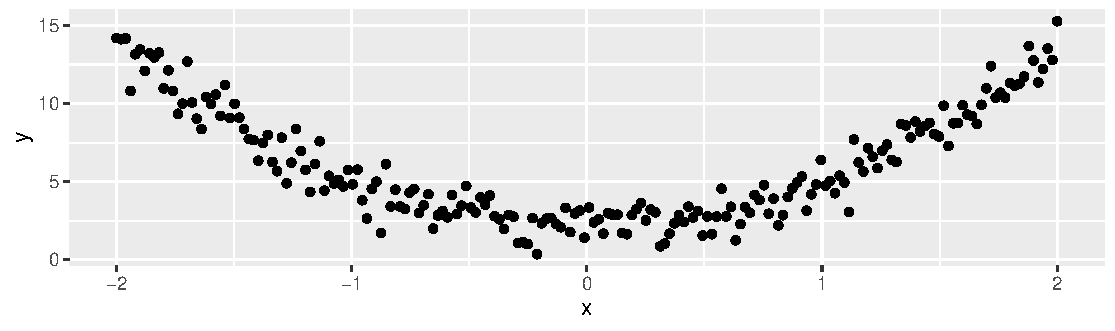
\includegraphics[width=6in]{parabola.pdf}
\eeqn

\noindent Let $X$ be the random variable (r.v.) that realized $x$ and let $Y$ be the r.v. that realized $y$.

\benum

\subquestionwithpoints{10} Record the letters of all the following that are \textbf{true}. Your answer will consist of a string (e.g. \texttt{aebgd}) where the order of the letters does not matter.

\begin{enumerate}[(a)]
\item $X$ and $Y$ are likely independent.
\item $X$ and $Y$ are likely dependent.
\item $X$ and $Y$ are likely associated.
\item $X$ and $Y$ are likely not associated.
\item $X$ and $Y$ likely have covariance zero.
\item $X$ and $Y$ likely have covariance nonzero.
\item $X$ and $Y$ likely have correlation zero.
\item $X$ and $Y$ likely have correlation nonzero.
\item If all values of $x > 0$ were dropped from $\mathbb{D}$, then it would appear that $X$ and $Y$ likely have covariance positive.
\item If all values of $x > 0$ were dropped from $\mathbb{D}$, then it would appear that $X$ and $Y$ likely have covariance negative.
\end{enumerate}
\eenum\pagebreak

\problem [13min] The raw $\mathbb{D}$ with $n = 27$ is plotted below where $x_1$ is on the horizontal axis and $x_2$ is on the vertical axis. The binary response $y$ measures patient outcome and is depicted by different shapes (see the illustration's legend).

\beqn
\centering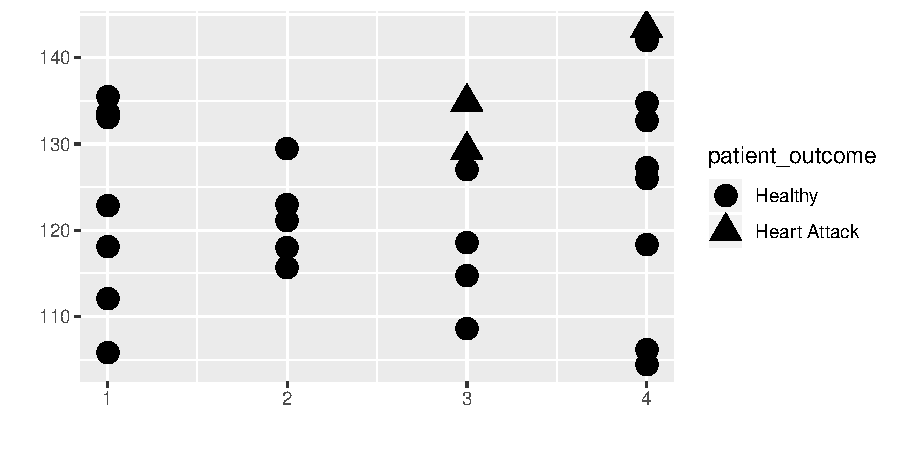
\includegraphics[width=5in]{nonlinsep.pdf}
\eeqn

\benum

\subquestionwithpoints{10} Record the letters of all the following that are \textbf{true}. Your answer will consist of a string (e.g. \texttt{aebgd}) where the order of the letters does not matter.

\begin{enumerate}[(a)]
\item $x_1$ is most likely an ordinal variable.
\item $x_1$ is most likely a nominal variable.
\item If $\mathcal{A} =$ OLS, then it would not be able to return a $g$.
\item If $\mathcal{A} =$ perceptron learning algorithm without a limit on iterations, then it would not be able to return a $g$.
\item If $\mathcal{A} =$ SVM with the Vapnik function, then you would need to specify the value of $\lambda$ to be able to return a $g$.
\item If $\mathcal{A} =$ SVM with the Vapnik function, then $g$ would have zero average hinge error.
\item If $\mathcal{A} =$ SVM with the Vapnik function and $\lambda = 0$, then $g$ would divide $\mathbb{D}$ only by using $x_1$.
\item Regardless of the $\mathcal{A}$ used, $R^2$ would be a preferred metric to assess model accuracy.
\item It is possible to design an $\mathcal{A}$ that could return a model $g$ that gives a perfect fit.
\item It $\mathcal{A} =$ KNN where $K = n$, then $g(\x)$ will be the same for all observations $\x \in \mathbb{D}$.
\end{enumerate}
\eenum\pagebreak

\problem [15min] A raw $\mathbb{D}$ is plotted below:

\beqn
\centering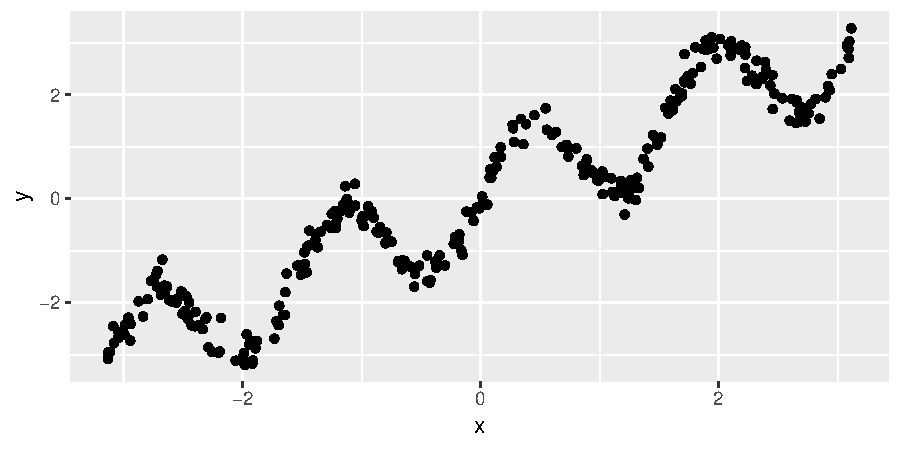
\includegraphics[width=5in]{curvyline.pdf}
\eeqn

\benum

\subquestionwithpoints{10} Record the letters of all the following that are \textbf{true}. Your answer will consist of a string (e.g. \texttt{aebgd}) where the order of the letters does not matter.

\begin{enumerate}[(a)]
\item $\mathcal{X}$ is likely $\bracks{-2,2}$.
\item $\mathcal{Y}$ is likely $\subseteq \reals$.
\item If $\mathcal{H} = \braces{a~:~a \in \reals}$ then a rational $\mathcal{A}$ would return $g$ where $a \approx 0$.
\item If $\mathcal{H} = \braces{a + b \indic{x > 0}\,:\,a,b \in \reals}$ then it is likely $f \in \mathcal{H}$.
\item If $\mathcal{H} = \braces{a + b \indic{x > 0}\,:\,a,b \in \reals}$ then a rational $\mathcal{A}$ would return $g$ where $b > a$.
\item If $\mathcal{H} = \braces{a + b \indic{x > 0}\,:\,a,b \in \reals}$ and $\mathcal{A} =$ OLS, then it would be impossible to compute $R^2$ for $g$.
\item If $\mathcal{H} =$ the space of all continuous functions, then $t \in \mathcal{H}$.
\item If $\mathcal{H} = \braces{a + b x\,:\,a,b \in \reals}$ then a rational $\mathcal{A}$ would return $g$ where $a < 0$.
\item With $\mathcal{H}$ specified optimally, the error due to estimation will likely be low.
\item With $\mathcal{H}$ specified optimally, the error due to misspecification will likely be low.
\end{enumerate}
\eenum\pagebreak



\problem [17min] Let $\X = \bracks{\onevec_n~|~\x_1~|~\ldots~|~\x_p} \in \reals^{n \times (p +1)}$ and $\rank{\X} = p + 1$ and $\y \in \reals^n$. Assume that the vectors $\x_1, \ldots, \x_p$ are mean-centered (i.e. the sample average of all their entries is zero) and that $\y$ is also mean-centered. Your modeling task is to model the response using the $n$ observations. Your $\mathcal{A} =$ OLS. Let $\b$ be the vector of OLS estimates for the $p+1$ features, let $\bbeta$ be the slope coefficients in the optimal linear model, $\H$ be the orthogonal projection matrix onto the $\colsp{\X}$, $\yhat$ is the vector of predictions for the $n$ observations and $\e$ are the residuals.

\benum

\subquestionwithpoints{10} Record the letters of all the following that are \textbf{true}. Your answer will consist of a string (e.g. \texttt{aebgd}) where the order of the letters does not matter.

\begin{enumerate}[(a)]
\item $\b = \displaystyle\argmin_{\w \in \reals^{p + 1}}\braces{(\y - \X\w)^\top (\y - \X\w)}$.
\item $\XtX$ is a full rank $n \times n$ matrix.
\item $\H$ is a full rank $n \times n$ matrix.
\item $\H\e = \zerovec_n$.
\item $\H\X\b - \yhat = \zerovec_n$.
\item $\H\X\bbeta - \yhat = \zerovec_n$.
\item $\onevec_n^\top\H\onevec_n = p + 1$.
\item $\x_2^\top\H\x_2 = (n - 1)s^2_{x_2}$.
\item $\rank{\I - \H} = n - p - 1$.
\item If $p = 0$ then $\yhat = \zerovec_n$.
\end{enumerate}
\eenum\pagebreak



\problem [13min] We use the same setup as in Problem 6. \ingray{Let $\X = \bracks{\onevec_n~|~\x_1~|~\ldots~|~\x_p} \in \reals^{n \times (p +1)}$ and $\rank{\X} = p + 1$ and $\y \in \reals^n$. Assume that the vectors $\x_1, \ldots, \x_p$ are mean-centered (i.e. the sample average of all their entries is zero) and that $\y$ is also mean-centered. Your modeling task is to model the response using the $n$ observations. Your $\mathcal{A} =$ OLS. Let $\b$ be the vector of OLS estimates for the $p+1$ features, let $\bbeta$ be the slope coefficients in the optimal linear model, $\H$ be the orthogonal projection matrix onto the $\colsp{\X}$, $\yhat$ is the vector of predictions for the $n$ observations and $\e$ are the residuals.} But now we progressively add columns consisting of entries of random noise to the matrix $\X$ which remains full rank each time a column is appended.

\benum

\subquestionwithpoints{10} Record the letters of all the following that are \textbf{true}. Your answer will consist of a string (e.g. \texttt{aebgd}) where the order of the letters does not matter. \\
~\\
With each additional column appended, ...

\begin{enumerate}[(a)]
\item SST decreases.
\item $\normsq{\yhat}$ increases.
\item $\dim\bracks{\H}$ remains the same.
\item $\rank{\H}$ remains the same.
\item the RMSE increases.
\item the generalization error of the model increases.
\item each residual's absolute value will decrease.
\item each slope coefficient (the entries in $\b$) will decrease.
\item the angle between $\yhat$ and $\y$ gets closer to zero.
\item with $p > n$, $\mathcal{A}$ fails to run.
\end{enumerate}
\eenum\pagebreak

\problem [12min] We use the same setup as in Problem 6. \ingray{Let $\X = \bracks{\onevec_n~|~\x_1~|~\ldots~|~\x_p} \in \reals^{n \times (p +1)}$ and $\rank{\X} = p + 1$ and $\y \in \reals^n$. Assume that the vectors $\x_1, \ldots, \x_p$ are mean-centered (i.e. the sample average of all their entries is zero) and that $\y$ is also mean-centered. Your modeling task is to model the response using the $n$ observations. Your $\mathcal{A} =$ OLS. Let $\b$ be the vector of OLS estimates for the $p+1$ features, let $\bbeta$ be the slope coefficients in the optimal linear model, $\H$ be the orthogonal projection matrix onto the $\colsp{\X}$, $\yhat$ is the vector of predictions for the $n$ observations and $\e$ are the residuals.} But now we use Q-R decomposition to find matrices such that $\X = \Q\R$ where $\q_j$ denotes the $j$th column of $\Q$.

\benum

\subquestionwithpoints{10} Record the letters of all the following that are \textbf{true}. Your answer will consist of a string (e.g. \texttt{aebgd}) where the order of the letters does not matter. 

\begin{enumerate}[(a)]
\item The dimension of $\Q$ is the same as $\X$.
\item $\colsp{\X} = \colsp{\Q}$.
\item $\R$ is a full rank $n \times n$ matrix.
\item $\R$ cannot be inverted.
\item $\y \in \colsp{\Q}$.
\item $\yhat \in \colsp{\Q}$.
\item The first column of $\Q$ is a scalar multiple of $\onevec_n$.
\item The last column of $\Q$ is a scalar multiple of $\x_p$.
\item $\H = \Q\Q^\top$.
\item $\yhat = \proj{\q_1}{\y} + \proj{\q_2}{\y} + \ldots + \proj{\q_{p+1}}{\y}$
\end{enumerate}
\eenum\pagebreak


\problem [14min] A dataset of $n = 40$ and $p=1$ is collected. Here is a plot of the raw $\mathbb{D}$:

\beqn
\centering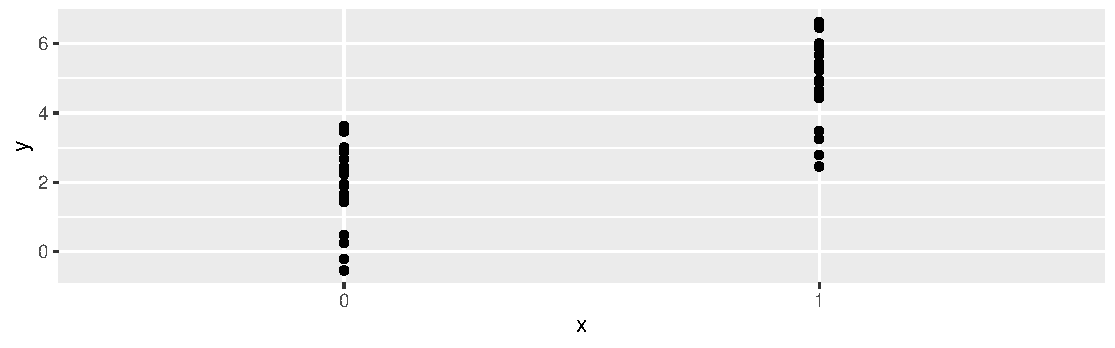
\includegraphics[width=6in]{binary.pdf}
\eeqn

And here is some \texttt{R} code that uses the raw $\mathbb{D} = \angbraces{\x,\y}$ with its output:

\begin{lstlisting}
> round(summary(y[x == 0]), 2)
   Min. 1st Qu.  Median    Mean 3rd Qu.    Max. 
  -0.54    1.47    1.91    1.86    2.72    3.63 
> round(summary(y[x == 1]), 2)
   Min. 1st Qu.  Median    Mean 3rd Qu.    Max. 
   2.46    4.47    4.91    4.86    5.72    6.63 
> mod = lm(y ~ x)
\end{lstlisting}
\vspace{-1cm}
\benum

\subquestionwithpoints{10} Record the letters of all the following that are \textbf{true}. Your answer will consist of a string (e.g. \texttt{aebgd}) where the order of the letters does not matter.

\begin{enumerate}[(a)]
\item $x$ is termed a ``dummy variable''.
\item Modeling the response $y$ here is termed a \qu{classification problem}.
\item The model $g$ in the object \texttt{mod} is a linear model.
\item The $R^2$ is likely to be low for the model $g$ in the object $\texttt{mod}$.
\item The $R^2$ is likely to be high for the model $g$ in the object $\texttt{mod}$.
\item When \texttt{coef(mod)} is called, it returns $b_1 = 4.86$.
\item When \texttt{coef(mod)} is called, it returns $b_1 = 3.00$.
\item If \texttt{mod = lm(y $\sim$ 0 + x)} and \texttt{coef(mod)} is called, it returns $b_1 = 4.86$.
\item If \texttt{mod = lm(y $\sim$ 0 + x)} and \texttt{coef(mod)} is called, it returns $b_1 = 3.00$.
\item The model $g$ in the object $\texttt{mod}$ can only predict for $x \in \braces{0,1}$.
\end{enumerate}
\eenum\pagebreak


\end{document}

\problem We are trying to predict heart attacks based on two risk factors: blood pressure and cholesterol. 

Blood pressure levels are based on the classification recommended by the Seventh Report of the Joint National Committee on Prevention, Detection, Evaluation and Treatment of High Blood Pressure and are defined as follows: normal (systolic blood pressure $<$120 mm Hg and a diastolic blood pressure $<$80 mm Hg); pre-hypertension (systolic blood pressure 120--139 mm Hg or diastolic blood pressure 80--89 mm Hg); hypertension stage 1 (systolic blood pressure 140--159 mm Hg or diastolic blood pressure 90--99 mm Hg); and hypertension stage 2 (systolic blood pressure $>$160 mm Hg or diastolic blood pressure $>$100 mm Hg). Persons are classified into the higher blood pressure group if the systolic and diastolic values fall within more than one category. Cholesterol is measured as the LDL cholesterol. 

Below is a plot of some historical pilot data.

\begin{figure}[htp]
\centering
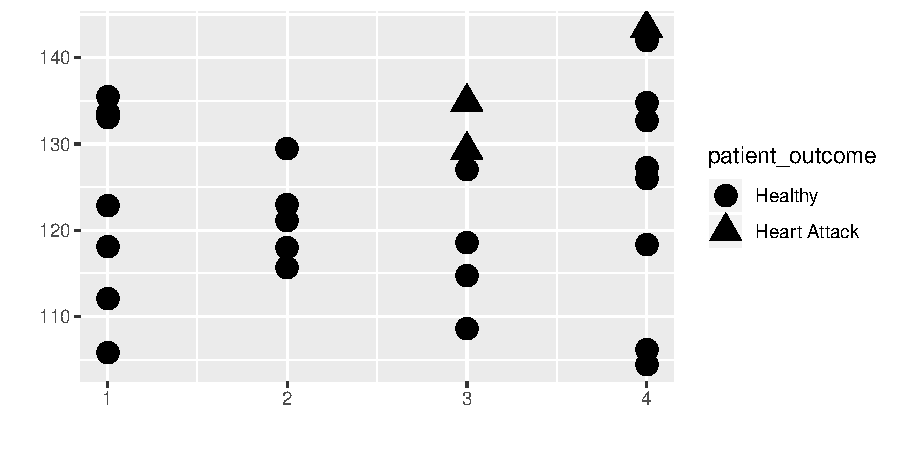
\includegraphics[width=6in]{nonlinsep}
\end{figure}

\benum
\subquestionwithpoints{2} Based on the description in the problem header label the axes  above. \spc{-0.5}


\subquestionwithpoints{2} If we are going to build a model from this data, what type of statistical learning are we doing? Circle all that apply.

\begin{enumerate}[i)]
\item regression to predict $y$
\item binary classification to predict $y$
\item multiclass (i.e. specifically non-binary) classification to predict $y$
\item finding $t$ directly
\item finding optimal $n$ and $p$ for $\mathbb{D}$
%\item building $\mathcal{A}$ to find $f$ directly
%\item estimating $\mathcal{X}$ and $\mathcal{Y}$ using $\mathcal{H}$
\item supervised learning
\item unsupervised learning
%\item OLS
\end{enumerate}

\subquestionwithpoints{2} Assume we are doing supervised learning. Relabel the axes and legend above using parentheses around $x_j$ and $y$ where $j$ is the index on the variable number which you need to determine. For example, an axis may be labeled \qu{\# of phone calls ($x_{17}$)}.

\subquestionwithpoints{2} Is this data linearly separable? Yes / no and explain your answer.\spc{2}

%\subquestionwithpoints{2} For the $x_j$'s and $y$ you named in the previous question, what are their types?\spc{2}

\subquestionwithpoints{2} Denote $\mathbb{D} := <X,\y>$. What is $\dim\bracks{X}$?

\subquestionwithpoints{2} Given $\mathbb{D}$, find $g_0$, the null model.\spc{-0.5}




\subquestionwithpoints{2} Let $\mathcal{A} = $ perceptron learning algorithm. What will its output be? Circle all that apply.

\begin{enumerate}[i)]
\item $\hat{y}$
\item $\mathcal{A}$
\item $g$
\item $h^*$
\item $x_{\cdot 1}, \ldots, x_{\cdot p}$
\item $f$
\item $z_1, \ldots, z_t$
\end{enumerate}

\subquestionwithpoints{4} Let $\mathcal{A} = $ perceptron learning algorithm. Starting the algorithm at the zero vector of the appropriate dimension, draw the algorithm's output line on the plot as a dotted line or explain below why you are unable to do so.\spc{3}


\subquestionwithpoints{2} Let $\mathcal{A} = $ an algorithm that minimizes average hinge loss. Write the objective function of the algorithm below.\spc{3}

\subquestionwithpoints{3} Let $\mathcal{A} = $  SVM with the Vapnik objective function with a $\lambda$ specified to be small but non-zero. Draw the algorithm's output line on the plot below or explain below why you are unable to do so.


\begin{figure}[htp]
\centering
\includegraphics[width=6in]{nonlinsep_trace}
\end{figure}

%\subquestionwithpoints{2} Is this $\mathcal{A}$ the same as using the SVM with the Vapnik objective function while setting $\lambda$ to be trivially small or zero? Yes / no.\spc{-0.5}

\subquestionwithpoints{2} What is the average classification error of the model in the previous question?\spc{1}

\subquestionwithpoints{2}  What is the approximate $R^2$ of this fit?

\begin{enumerate}[i)]
\item $<$0\%
\item 0\%
\item 2.5\%
\item 25\%
\item 95\%
\item 100\%
\item $\mathcal{A}$ cannot produce an output thus $R^2$ cannot be estimated.
\end{enumerate}

\subquestionwithpoints{2}  Why is $R^2$ an inappropriate metric to be using here to measure model performance?\spc{4}

%\subquestionwithpoints{2} Draw a $p=1$ threshold model below that has minimum average misclassification error.
%
%
%\begin{figure}[htp]
%\centering
%\includegraphics[width=6in]{nonlinsep_trace}
%\end{figure}



\subquestionwithpoints{2} Draw a model below that has zero average hinge error.


\begin{figure}[htp]
\centering
\includegraphics[width=6in]{nonlinsep_trace}
\end{figure}


\subquestionwithpoints{4} Let $\mathcal{A} = $ KNN with $d = $ Euclidean distance. Evaluate the following:

\begin{enumerate}[i)]
\item $K$ = 1, $g(4,145) = $
\item $K$ = 1, $g(3,125) = $ 
\item $K$ = 4, $g(3,125) = $ 
\end{enumerate}

\subquestionwithpoints{5} Is there a problem with using  $\mathcal{A} = $ perceptron, $\mathcal{A} = $ SVM and $\mathcal{A} = $ KNN with $\mathbb{D}$? Yes / no. Discuss.\spc{10}
\eenum

\problem The following dataset is a mock view of a financial asset. The $x$ axis represents time and the $y$ axis represents value. There are $n = 300$ data points and $s^2_x = 3.322$ and $s^2_y = 3.196$.

\begin{figure}[htp]
\centering
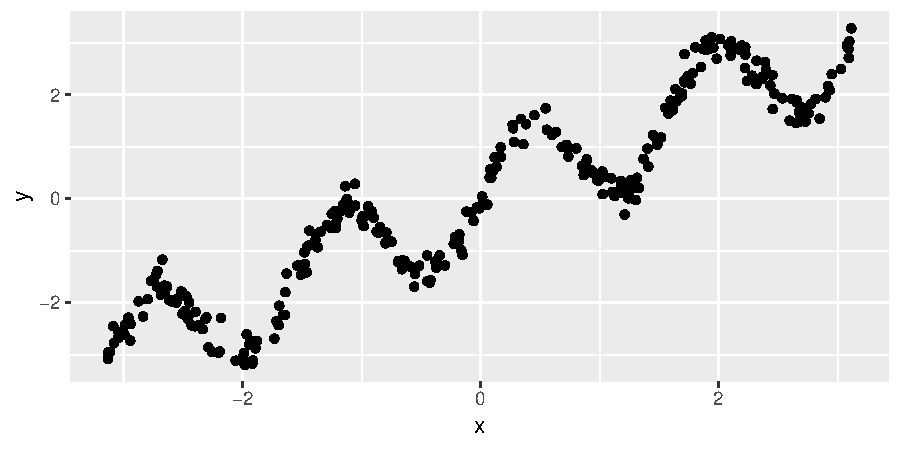
\includegraphics[width=5in]{curvyline}
\end{figure}


\benum

\subquestionwithpoints{2} Estimate $\mathcal{X}$ and $\mathcal{Y}$.\spc{0.5}
\subquestionwithpoints{2} Estimate the equation for $g_0$.\spc{0}

\subquestionwithpoints{2} Estimate the $R^2$ for $g_0$.\spc{0}

%\subquestionwithpoints{2} If $\mathcal{A} = $ OLS, estimate the equation for $g$.\spc{1}

\subquestionwithpoints{5} If $\mathcal{A} = $ OLS, estimate the percentage of the RMSE of $g$ belonging to each of the three errors. 

\begin{enumerate}[i)]
\item Name of error:\\
~\\
Percentage of RMSE:\\
\item Name of error:\\
~\\
Percentage of RMSE:\\
\item Name of error:\\
~\\
Percentage of RMSE:\\
\end{enumerate}


%\subquestionwithpoints{2} If $\mathcal{A} = $ OLS, and $\x$ (the vector of all $x_i$'s) were drawn from the r.v. model $X$ and $\e$ (the vector of all $e_i$'s) were drawn from the r.v. model $E$, do you think $X$ and $E$ would be independent? Explain why or why not. \spc{2}

\subquestionwithpoints{4} Let $\mathcal{A} = $ minimize the least squares error but provide a better $\mathcal{H}$ than the set $\braces{w_0 + w_1 x~:~w_0, w_1 \in \reals}$ where \qu{better} means that the elements $h$ can much better approximate $f$. \spc{1}


\subquestionwithpoints{2} Draw $h^*$, an element of your set in (d) on the plot below:

\begin{figure}[htp]
\centering
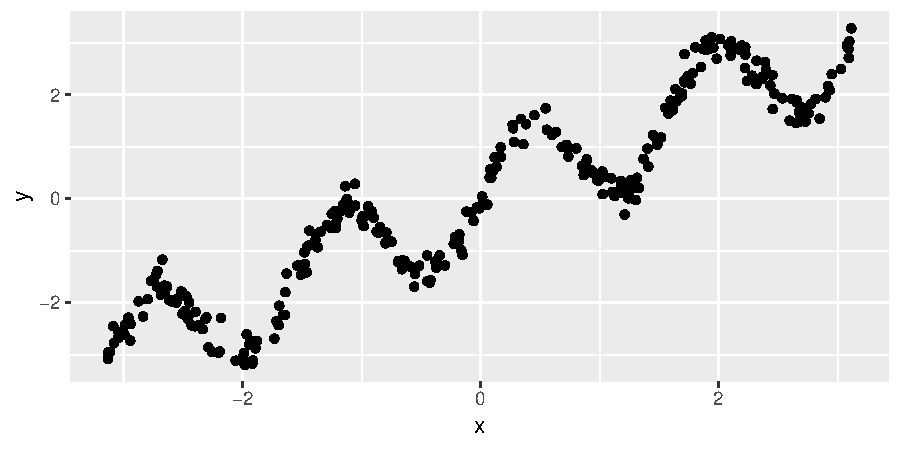
\includegraphics[width=5in]{curvyline}
\end{figure}


\subquestionwithpoints{5} Compute the $R^2$ of the model depicted as the solid line below \emph{as best as you can}.

\begin{figure}[htp]
\includegraphics[width=5in]{curvyline_with_f}
\end{figure}~\spc{4}


\eenum

\problem We will now be looking at the \texttt{diamonds} dataset. Below is some \texttt{R} code that gives background on this data frame which will be referenced throughout this problem. The response variable that is usually modeled is \texttt{price}. This problem contains some coding exercises. 

\lstset{basicstyle=\scriptsize}
\begin{lstlisting}
> diam = ggplot2::diamonds
> dim(diamonds)
[1] 53940    10
> summary(diamonds)
     carat               cut        color        clarity          depth      
 Min.   :0.2000   Fair     : 1610   D: 6775   SI1    :13065   Min.   :43.00  
 1st Qu.:0.4000   Good     : 4906   E: 9797   VS2    :12258   1st Qu.:61.00  
 Median :0.7000   Very Good:12082   F: 9542   SI2    : 9194   Median :61.80  
 Mean   :0.7979   Premium  :13791   G:11292   VS1    : 8171   Mean   :61.75  
 3rd Qu.:1.0400   Ideal    :21551   H: 8304   VVS2   : 5066   3rd Qu.:62.50  
 Max.   :5.0100                     I: 5422   VVS1   : 3655   Max.   :79.00  
                                    J: 2808   (Other): 2531                  
     table           price             x                y                z         
 Min.   :43.00   Min.   :  326   Min.   : 0.000   Min.   : 0.000   Min.   : 0.000  
 1st Qu.:56.00   1st Qu.:  950   1st Qu.: 4.710   1st Qu.: 4.720   1st Qu.: 2.910  
 Median :57.00   Median : 2401   Median : 5.700   Median : 5.710   Median : 3.530  
 Mean   :57.46   Mean   : 3933   Mean   : 5.731   Mean   : 5.735   Mean   : 3.539  
 3rd Qu.:59.00   3rd Qu.: 5324   3rd Qu.: 6.540   3rd Qu.: 6.540   3rd Qu.: 4.040  
 Max.   :95.00   Max.   :18823   Max.   :10.740   Max.   :58.900   Max.   :31.800
\end{lstlisting}

\lstset{basicstyle=\footnotesize}

\benum

\subquestionwithpoints{2} In this $\mathbb{D}$, what is $n$ and $p$? \spc{0}

\subquestionwithpoints{2} What is the type of the variable \texttt{carat}? \spc{0}

\subquestionwithpoints{2} What is the type of the variable \texttt{cut}? \spc{0}

\subquestionwithpoints{2} If you were fitting an OLS model of \texttt{price} using \texttt{color}, what would $p$ be in that model? \spc{0}

\subquestionwithpoints{2} Write code that extracts every 50th diamond observation. \spc{1}

\subquestionwithpoints{3} Write code that adds a new variable to the data frame named \texttt{customer\_favorite} that is 1 if the \texttt{cut} is \texttt{ideal} and the \texttt{color} is either \texttt{G} or \texttt{J} and the \texttt{depth} is 90\%ile or above. \spc{3}

\subquestionwithpoints{3} Assume that \texttt{x}, \texttt{y} and \texttt{z} are the spatial dimensions of the stone. Write code below that creates a data frame called \texttt{tinies} that contains diamonds that have volume less than 50. \spc{0.5}

\subquestionwithpoints{3} Describe the output of this script as completely as possible.

\begin{lstlisting}
> dict = list()
> for (color in unique(diam$color)){
  dict[[color]] = diam[diam$color == color, "price"]
}
> dict[["D"]]
\end{lstlisting}~\spc{1.5}

\eenum


\problem This last problem contains a pure coding exercise. 

\benum

\subquestionwithpoints{5} Complete the function below to spec. You don't have to use all the free lines given (in fact, it can be done in one line). You are free to use the \texttt{mean}, \texttt{sd}, \texttt{cov}, \texttt{cor} and other base \texttt{R} functions (but you cannot use \texttt{lm}). \spc{-0.5}

\begin{lstlisting}
#' This function implements the linear least squares regression algorithm
#' for one covariate popularized by Sir Francis Galton in 1886.
#'
#' @param x		the continuous predictor
#' @param y		the continuous response 	
#' @return 		a list containing a key ``b_0'' whose value is the inter-
#'						cept, a key ``b_1'' whose value is the slope, a key ``Rsq''
#'						that is the R-squared of the fit.
linear_least_squares_algorithm = function(x, y){
  b_1 = cor(x, y) * sd(y) / sd(x)
  b_0 = mean(y) - b_1 * mean(x)











}
\end{lstlisting}

\eenum
\end{document}

